\documentclass[conference]{IEEEtran}
\usepackage{amsmath,amssymb,graphicx,booktabs,cite}
\usepackage[T1]{fontenc}
\usepackage{microtype}
\usepackage{array}
\setlength{\emergencystretch}{2em}
\hyphenation{re-ver-be-ra-tion cen-so-ring}

\begin{document}

\title{Automatic-Censoring K-Distribution CFAR Detection for Active Sonar in Heavy-Tailed Reverberation}

\author{\IEEEauthorblockN{Mohammed Tausif Abdullah}
\IEEEauthorblockA{Department of Electronics and Communication Engineering\\
Chaitanya Bharathi Institute of Technology, Hyderabad, India\\
Email: juniorscientist3@gmail.com}}

\maketitle

\begin{abstract}
Constant false alarm rate (CFAR) detectors used in active sonar are usually designed for Gaussian backgrounds, yet sonar reverberation is heavy-tailed, and reference windows are further corrupted by interfering targets and reverberation edges. We study CFAR behaviour under K-distributed reverberation and propose ACK-CFAR, which combines a log-moment estimate of the K shape parameter with model-based automatic censoring and an estimator-aware threshold. Monte Carlo simulations show that CA-, OS- and VI-CFAR exceed the design false-alarm probability by roughly 16--25 times in spiky homogeneous reverberation, while the calibrated ACK-CFAR reduces the excess to about 3 times, and to about 1 time in the presence of three interfering targets. The price is a detection loss of 1--2 dB relative to classical detectors at matched false-alarm probability, caused mainly by shape estimation from a short window. We discuss this trade-off and outline how longer-window shape estimation may close the gap.
\end{abstract}

\begin{IEEEkeywords}
active sonar, CFAR, K-distribution, reverberation, automatic censoring
\end{IEEEkeywords}

\section{Introduction}
Active sonar detection relies on adaptive thresholds that keep the false-alarm rate constant as the background changes. Classical mean-level and order-statistic detectors (CA, GO, SO, OS)~\cite{finn1968,rohling1983} assume a Gaussian (exponential-intensity) background. In practice, sonar reverberation departs from the Rayleigh model toward heavy-tailed distributions such as log-normal, Weibull and K~\cite{zhang2017}. K-distribution based CFAR has been proposed for sonar imagery~\cite{abu2020}, variability-index CFAR has been extended to multistatic sonar~\cite{vi_sonar}, and recent work combines segmentation with local CFAR~\cite{sow2025}.

We ask a narrower question: how do standard detectors behave when heavy-tailed reverberation, interfering targets and reverberation edges occur together, and can a K-model detector with automatic censoring control false alarms better? Our contributions are (i) a controlled simulation comparison of CA, GO, SO, OS, VI and K-model detectors in these conditions, (ii) ACK-CFAR, and (iii) an honest account of the detection-loss cost.

\section{Signal Model}
The reverberation intensity in a cell is $I=\tau E$, where $E\sim\mathrm{Exp}(1)$ is speckle and $\tau\sim\mathrm{Gamma}(\nu,\mu/\nu)$ is texture, giving the K-distribution with shape $\nu$ and mean $\mu$. The tail is
\begin{equation}
P(I>t)=\frac{2}{\Gamma(\nu)}\left(\frac{\nu t}{\mu}\right)^{\nu/2}K_\nu\!\left(2\sqrt{\nu t/\mu}\right).
\end{equation}
Small $\nu$ means spiky reverberation; $\nu\to\infty$ recovers the Gaussian case. A Swerling-I target of signal-to-clutter ratio (SCR) adds $\mathrm{SCR}\cdot\mu$ to the texture of the cell under test (CUT). We use a reference window of $2\times16$ cells with 2 guard cells per side.

\section{Detectors}
\subsection{Baselines}
CA, GO, SO and OS ($k=3N/4$) thresholds are designed for exponential background (scale factors by closed form or Monte Carlo). VI-CFAR switches among CA, GO and SO using variability-index and mean-ratio tests~\cite{smith2000}. K-LM estimates $(\nu,\mu)$ by log-moments without censoring.

\subsection{Proposed ACK-CFAR}
Since $\mathrm{Var}[\ln I]=\psi_1(\nu)+\pi^2/6$, the shape is obtained by inverting the trigamma function on the sample variance of $\ln I$ over retained reference cells. Cells above $c(\hat\nu)\hat\mu$ are censored, where $c(\cdot)$ is the K-tail quantile at a small probability $p_c$; because $c$ grows for spiky reverberation, genuine clutter spikes are kept while strong interferers are removed. The mean of retained cells is corrected for truncation, and the procedure is iterated twice. ACK-CFAR uses the analytic K threshold $\kappa(\hat\nu)\hat\mu$; ACK-cal replaces $\kappa$ by a Monte Carlo learned function of $\hat\nu$, accounting for estimation noise.

\section{Simulation Setup}
Scenarios: homogeneous reverberation; three interferers at 15~dB inside the reference window; and a 10~dB reverberation edge with the CUT on the high or low side. Shape values $\nu\in\{1,3,\infty\}$. Design $P_{fa}=10^{-3}$, $10^6$ trials for $P_{fa}$ and $2\times10^4$ per SCR point for $P_d$. Detectors are also compared at \emph{matched} $P_{fa}$ by setting each detector's threshold to its own empirical $(1-P_{fa})$ quantile. An oracle with known $(\nu,\mu)$ gives a bound. Code is available from the authors.

\section{Results}
Fig.~\ref{fig:pd} shows $P_d$ against SCR at matched $P_{fa}$ for $\nu=1$, Fig.~\ref{fig:pfa} the measured $P_{fa}$ for all detectors, and Table~\ref{tab:res} the measured $P_{fa}$ (as a multiple of the design value) together with the SCR required for $P_d=0.9$ at matched $P_{fa}$.

\begin{figure*}[!t]
\centering
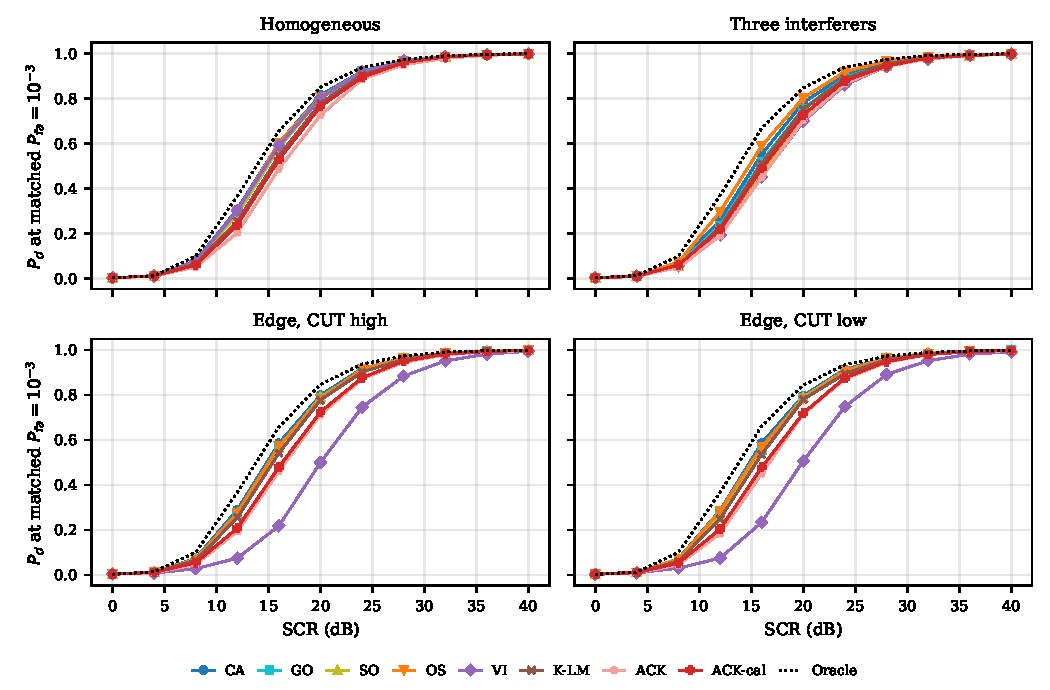
\includegraphics[width=0.86\textwidth]{figures/fig_pd_nu1.pdf}
\caption{$P_d$ versus SCR at matched $P_{fa}=10^{-3}$ for $\nu=1$ in the four scenarios.}
\label{fig:pd}
\end{figure*}

\begin{figure*}[!t]
\centering
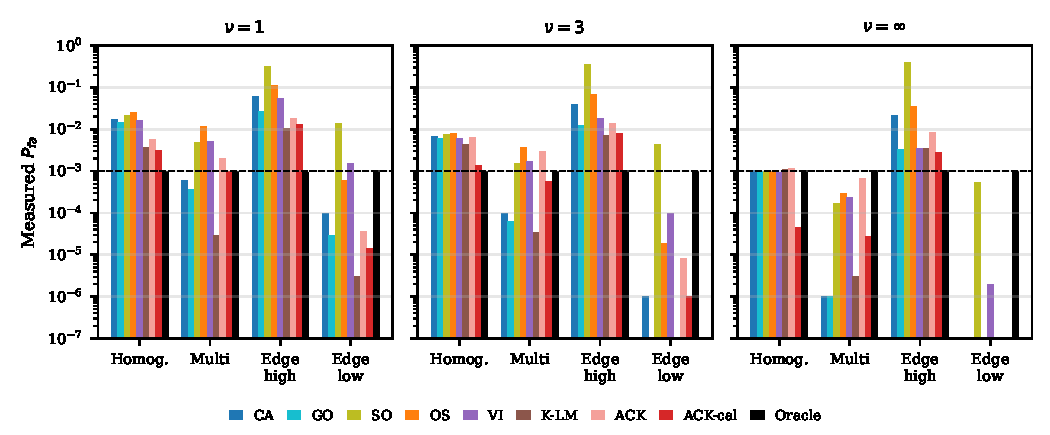
\includegraphics[width=0.92\textwidth]{figures/fig_pfa.pdf}
\caption{Measured $P_{fa}$ against the design value $10^{-3}$ (dashed) for all detectors and scenarios.}
\label{fig:pfa}
\end{figure*}

\begin{table*}[!t]
\centering
\caption{Measured $P_{fa}$ as a multiple of the design value ($10^{-3}$) / SCR (dB) for $P_d=0.9$ at matched $P_{fa}$}
\label{tab:res}
\scriptsize
\setlength{\tabcolsep}{3.6pt}
\begin{tabular}{@{}cl*{9}{c}@{}}
\toprule
$\nu$ & Scenario & CA & GO & SO & OS & VI & K-LM & ACK & ACK-cal & Oracle \\
\midrule
$1$ & Homog. & 17/23.2 & 14/23.3 & 21/23.6 & 24/23.4 & 16/23.4 & 3.7/23.9 & 5.8/24.9 & 3.1/24.4 & 1.0/22.3 \\
 & 3 interf. & 0.6/24.0 & 0.4/24.5 & 4.9/25.6 & 12/23.4 & 5.1/25.9 & 0.0/24.8 & 2.0/25.8 & 1.0/25.3 & 1.0/22.3 \\
 & Edge hi & 59/23.4 & 27/23.8 & 314/23.8 & 112/23.6 & 55/29.0 & 11/23.9 & 18/25.6 & 13/25.3 & 0.9/22.4 \\
 & Edge lo & 0.1/23.5 & 0.0/23.8 & 13/23.7 & 0.6/23.8 & 1.5/28.6 & 0.0/24.4 & 0.0/25.6 & 0.0/25.4 & 1.0/22.5 \\
\midrule
$3$ & Homog. & 6.8/21.0 & 6.0/21.2 & 7.3/21.3 & 8.0/21.3 & 6.1/21.1 & 4.4/22.1 & 6.4/22.7 & 1.4/21.9 & 1.0/20.1 \\
 & 3 interf. & 0.1/22.6 & 0.1/23.1 & 1.5/23.3 & 3.6/21.4 & 1.7/23.6 & 0.0/23.8 & 2.9/23.3 & 0.6/22.5 & 1.0/20.3 \\
 & Edge hi & 40/21.5 & 12/21.6 & 353/21.7 & 68/22.1 & 18/24.5 & 7.2/22.6 & 14/23.9 & 8.0/23.2 & 1.1/20.4 \\
 & Edge lo & 0.0/21.4 & 0.0/21.6 & 4.4/21.7 & 0.0/22.0 & 0.1/24.2 & 0.0/22.6 & 0.0/23.8 & 0.0/23.3 & 1.0/20.1 \\
\midrule
$\infty$ & Homog. & 1.1/18.9 & 1.0/19.1 & 1.0/19.2 & 1.0/19.1 & 0.9/18.9 & 1.1/19.4 & 1.2/19.7 & 0.0/19.2 & 1.0/18.5 \\
 & 3 interf. & 0.0/21.0 & 0.0/21.7 & 0.2/21.8 & 0.3/19.1 & 0.2/22.1 & 0.0/23.2 & 0.6/20.3 & 0.0/19.7 & 1.0/18.4 \\
 & Edge hi & 22/19.2 & 3.2/19.3 & 394/19.3 & 35/19.8 & 3.4/19.5 & 3.4/20.4 & 8.3/22.5 & 2.8/21.5 & 1.1/18.5 \\
 & Edge lo & 0.0/19.2 & 0.0/19.3 & 0.5/19.4 & 0.0/19.9 & 0.0/19.5 & 0.0/20.5 & 0.0/22.5 & 0.0/21.4 & 1.0/18.4 \\
\bottomrule
\end{tabular}
\end{table*}

\noindent Oracle reference: $P_{fa}\approx1$ and SCR $\approx22.3$~dB in the homogeneous case. In Gaussian noise ($\nu=\infty$) all classical detectors hold the design $P_{fa}$, while ACK-cal is conservative.

Classical detectors designed for Gaussian noise exceed the design false-alarm rate by more than an order of magnitude in spiky reverberation. ACK-cal substantially reduces the excess, but at matched $P_{fa}$ it loses 1--2~dB against CA-type detectors, and more when the CUT lies on the low side of an edge. Most of the remaining gap to the oracle is due to estimating $\nu$ from 32 cells.

\section{Discussion and Limitations}
The advantage demonstrated is false-alarm control, not detection gain. The evaluation is synthetic with independent texture across cells, whereas real reverberation has correlated texture; K-LM is a simplified stand-in for published K-CFAR detectors; and no real sonar data were used. Future work: estimate shape over a long window or in 2-D, add explicit edge logic, and validate on measured data.

\section{Conclusion}
Heavy-tailed reverberation makes Gaussian-designed CFAR detectors unreliable in false-alarm control. Automatic censoring with a log-moment K model restores much of it at a modest detection cost, and shape-estimation accuracy is the main factor to improve.

\begin{thebibliography}{9}
\bibitem{finn1968} H.~M. Finn and R.~S. Johnson, ``Adaptive detection mode with threshold control as a function of spatially sampled clutter estimates,'' \emph{RCA Review}, vol.~29, pp.~414--464, 1968.
\bibitem{rohling1983} H.~Rohling, ``Radar CFAR thresholding in clutter and multiple target situations,'' \emph{IEEE Trans. Aerosp. Electron. Syst.}, vol.~AES-19, no.~4, pp.~608--621, 1983.
\bibitem{smith2000} M.~E. Smith and P.~K. Varshney, ``Intelligent CFAR processor based on data variability,'' \emph{IEEE Trans. Aerosp. Electron. Syst.}, vol.~36, no.~3, pp.~981--990, 2000.
\bibitem{abu2020} A.~Abu and R.~Diamant, ``CFAR detection algorithm for objects in sonar images,'' \emph{IET Radar Sonar Navig.}, 2020.
\bibitem{zhang2017} Zhang \emph{et al.}, ``Clutter-suppressing performance estimation methods of active sonar waveform based on reverberation statistical models in littoral environment,'' \emph{IET Radar Sonar Navig.}, 2017. [VERIFY authors]
\bibitem{vi_sonar} ``Robust centralized CFAR detection for multistatic sonar systems,'' [VERIFY authors, venue, year]
\bibitem{sow2025} ``A constant false alarm rate detection method for sonar imagery targets based on segmented ordered weighting,'' \emph{J. Mar. Sci. Eng.}, vol.~13, no.~4, 2025. [VERIFY authors]
\end{thebibliography}

\end{document}
